\subsection{Model}


Das Datenmodell des Radarsimulators wurde mit Hilfe des Frameworks EMF erstellt. Das Modell befindet sich in einem eigenen Plug-In Modul. Darin sind ein graphisches Entity-Relation-Diagramm des Modells und der daraus generierbare Modellcode enthalten. Das Objekt, welches die Informationen des Sensors zusammenfasst, heißt \texttt{SimulatorModelRadar}. Dieses enthält 19 Attribute, die die Eigenschaften des simulierten Sensors beschreiben. Zusätzlich gibt es noch Beziehungen zu zehn Klassen, die die Daten des Sensors speichern. Die Klassen, die in dieser Arbeit verwendet werden, sind:

\begin{itemize}
    \item \texttt{SimulatorBitNode}: Der \texttt{SimulatorBitNode} ist eine Baumdatenstruktur in der Bitfehler abgelegt werden. Das SimulatorModelRadar besitzt höchstens einen SimulatorBitNode.    
    \item \texttt{SimulatorModelDefectReport}: In der Liste der DefectReports werden Bitfehler von speziellen Sensoren gespeichert.
    \item \texttt{SimulatorModelEquipment}: Der SimulatorModelRadar kann beliebig viele SimulatorModelEquipment-Objekte des Sensors gespeichern. Weil die PNU ein Zubehör des Sensors ist, werden dessen Informationen als SimulatorModelEquipment gespeichert. Dafür gibt es die Klasse SimulatorModelPNU, welche SimulatorModelEquipment erweitert. 
    \item \texttt{SimulatorModelSector}: Um Sektor Informationen des Sensors zu speichern, gibt es die Klasse SimulatorModelSector. Die Klasse SimulatorModelRadar hat höchstens einen aktuellen Sektor und beliebig viele weitere Sektoren.    
\end{itemize}

Was bei der Betrachtung des grafischen Modells auffällt ist, dass es drei vom SimulatorModelRadar unabhängige Klassen gibt. Diese Klassen sind:

\begin{itemize}
    \item \texttt{Scenario}: Die Klasse Scenario beinhaltet beliebig viele ScenarioTargets, welche beliebig viele Waypoints haben. Man erkennt daran gut wie das Scenario aufgebaut ist. Die ScenarioTargets sind mögliche Objekt, die der Sensor detektieren kann. Das sind zum Beispiel Fußgänger oder PKWs. Diese Objekte bewegen sich auf einem Pfad, welcher durch die Waypoints (auf Deutsch Wegpunkte) definiert wird.
    \item \texttt{TargetSimulation}:  Die TargetSimulation beschreibt die Eigenschaften, wie z.B. Position, Klassifizierung und Radarquerschnitt, eines Radarziels zu einem bestimmten Zeitpunkt. Eine TargetSimulation entsteht, wenn im UI ein Scenario abgespielt wird. Dabei wird die aktuelle Position eines ScenarioTargets, anhand der Wegpunkte berechnet und daraus wird eine TargetSimulation erstellt.
    \item \texttt{SimulatorModelTrack}: Ein SimulatorModelTrack beschreibt ebenso, wie die TargetSimulation, die Eigenschaften eines Radarziels. Der entscheidende Unterschied ist, dass dieses Radarziel nun abhängig vom Sensor ist. Deswegen hat diese weitere Attribute, welche die Venus benötigt, um das Ziel darzustellen. In Tabelle \ref{table:1} werden die entscheidenden Unterschiede der beiden Klassen aufgezeigt.    
\end{itemize}

\begin{table}[h]
    \begin{tabular}{ |c|c|c| } 
        \hline
         & \texttt{TargetSimulation} & \texttt{SimulatorModelTrack} \\ 
        \hline
        Koordinatensystem & Lat/Long & Polarkoordinaten \\ 
        \hline
        Doppler Speed Informationen & - & x \\ 
        \hline
        Höhenangabe & über dem Meeresspiegel & relativ zum Sensor \\ 
        \hline
        Beamline-hitcount & - & x \\ 
        \hline
        Confidence des Ziels & - & x \\ 
        \hline        
   \end{tabular}
   \caption{Vergleich zwischen \texttt{TargetSimulation} und \texttt{SimulatorModelTrack}}
   \label{table:1}
\end{table}

Wie sinnvoll ist es nun diese Klassen vom Modell zu trennen? Das Scenario wird von der GUI-Komponente verwendet, um es auf einer Karte darzustellen und um es als XML-Datei zu speichern. Wie man in Abbildung \ref{figure:scenarioview} erkennen kann gehört das \texttt{Scenario} zum \texttt{ScenarioController} und lediglich der \texttt{ScenarioUpdater} ist vo ihm abhängig. Deswegen ist es nicht notwendig das \texttt{Scenario} im Modell zu speichern und es müssen keine Änderungen vorgenommen werden.

\begin{figure}[ht]
    \centering
    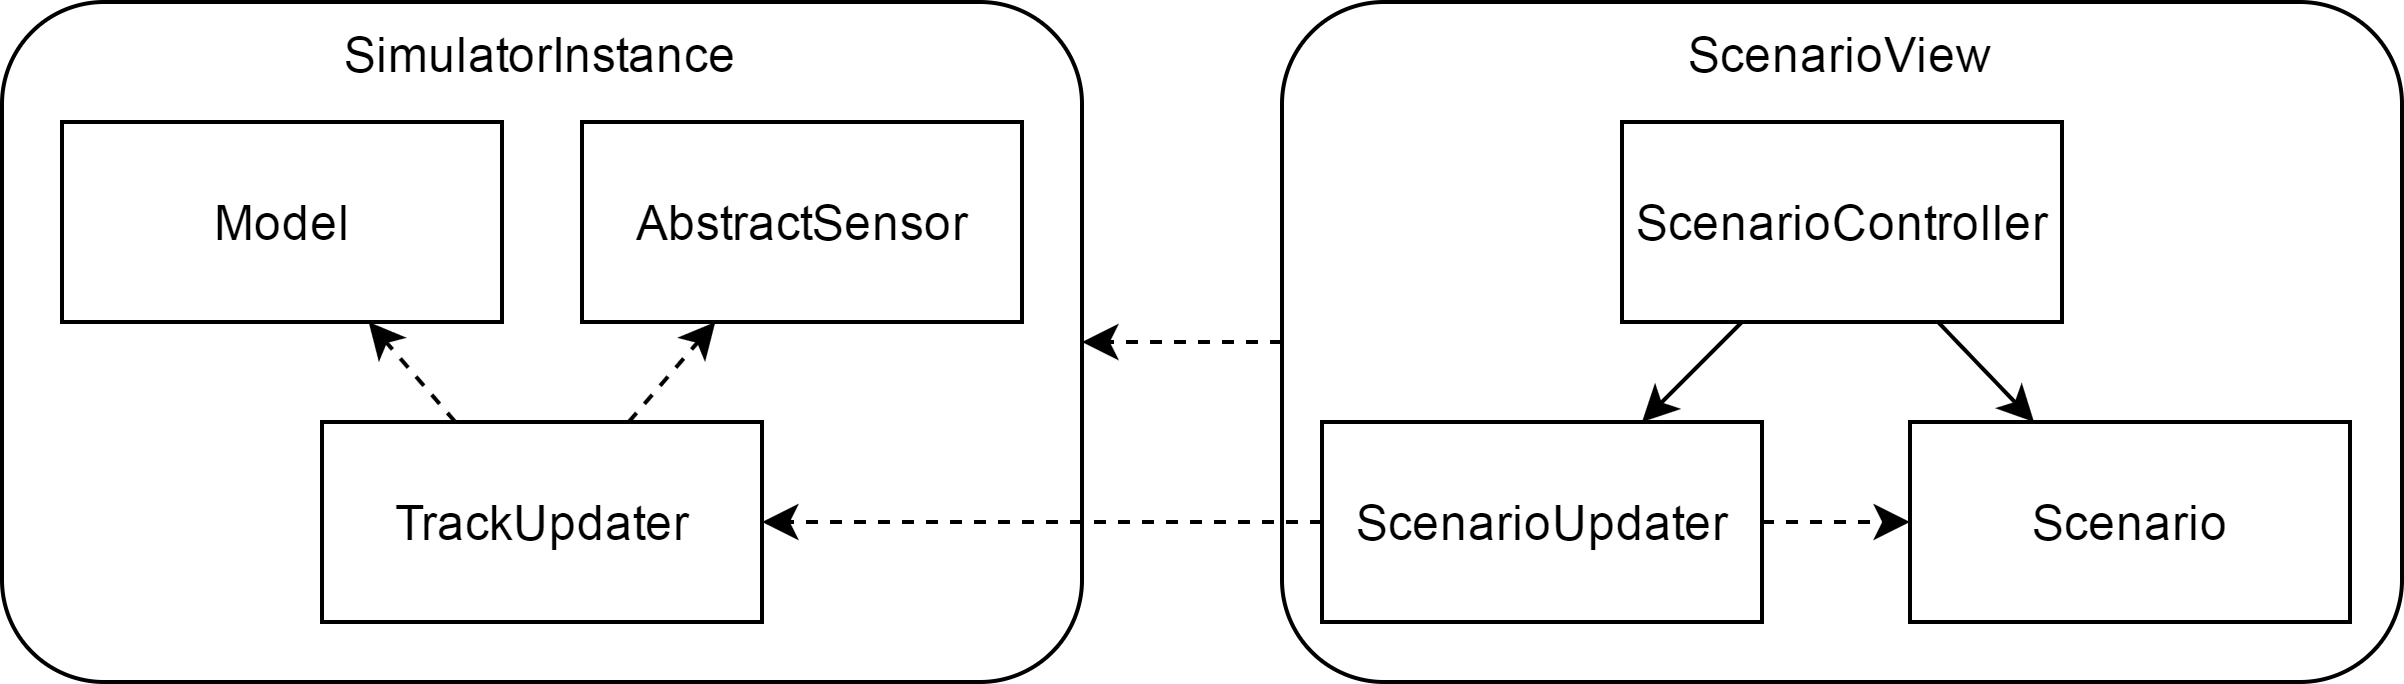
\includegraphics[width=1\textwidth]{content/assets/Kapitel3/ScenarioViewRelations.png}
    \caption{Beziehung zwischen SimulatorInstance und ScenarioView}
    \label{figure:scenarioview}
\end{figure}

\texttt{TargetSimulation-Objekte} werden nur vom \texttt{ScenarioUpdater} erzeugt. Dieser hat eine Liste mit \texttt{ITargetUpdateListener}, bei denen nach einem bestimmten Zeitintervall die Methode \texttt{updateTarget(Targetsimulation)} aufgerufen wird. Der \texttt{TrackUpdater} ist einer der \texttt{ITargetUpdateListener}. Die TargetSimulation-Objekte werden direkt durch den Methodenparameter an den \texttt{TrackUpdater} übergeben.

\begin{figure}[ht]
    \centering
    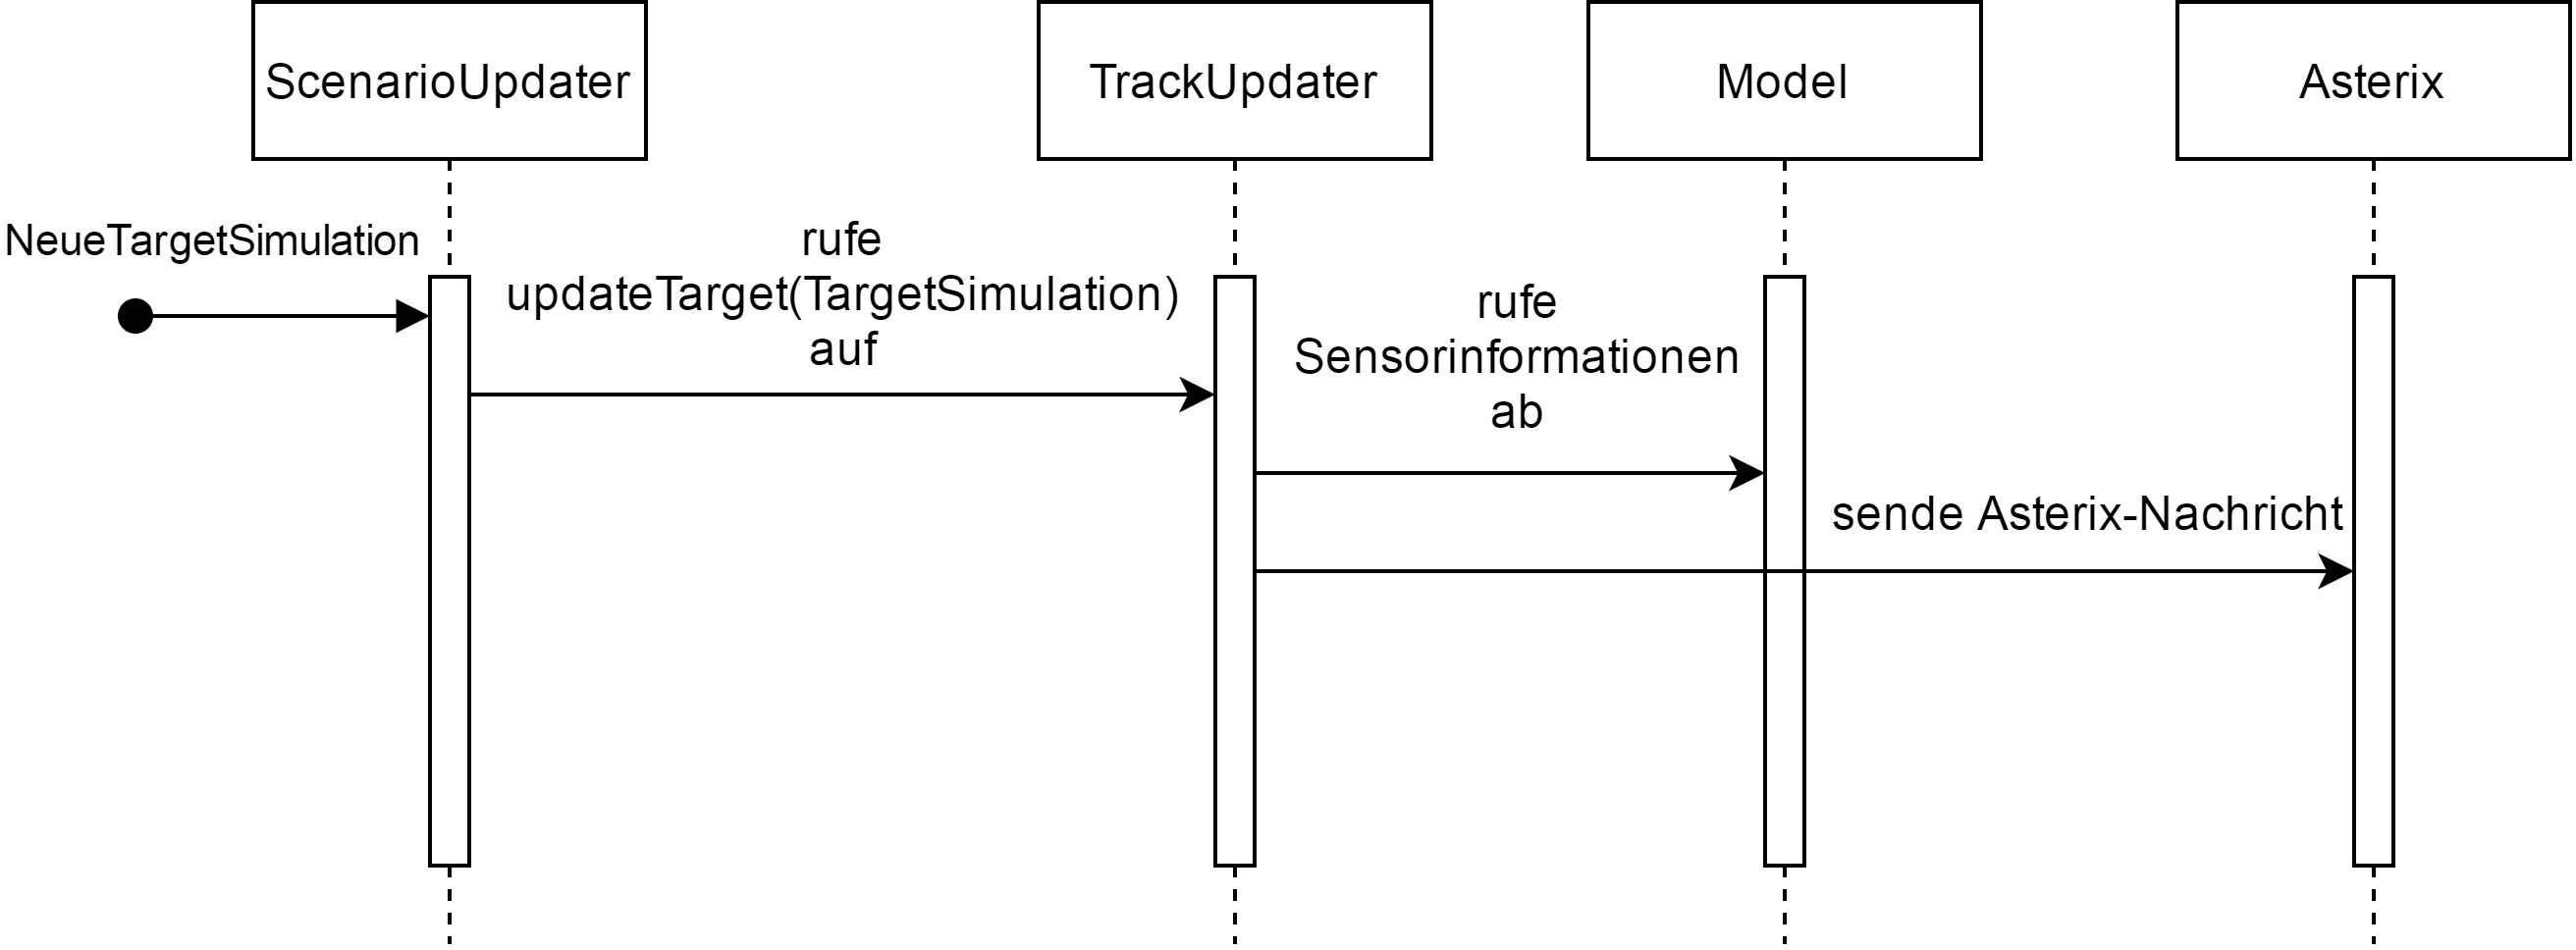
\includegraphics[width=1\textwidth]{content/assets/Kapitel3/TargetSimulationUsecase.png}
    \caption{Beziehung zwischen SimulatorInstance und ScenarioView}
    \label{figure:x}
\end{figure}

Eine modulare Architektur hat klare Schnittstellen. Das Problem ist aber, dass in diesem Fall die \texttt{SimulatorInstance} keine geeignete Schnittstelle ist zwischen der GUI-Komponente und . Im Fall der neuen Anwendung, soll die Schnittstelle zwischen \texttt{SimulatorInstance} und ScenarioView nicht mehr die gesamte \texttt{SimulatorInstance} sein, sondern im Optimalfall nur noch das Modell. Wenn aber das Modell die einzige Schnittstelle zwischen \texttt{SimulatorInstance} und View-Komponente ist, hat der ScenarioUpdater keinen Zugriff mehr auf den \texttt{TrackUpdater}.

Wie ist es nun möglich, dass der ScenarioUpdater die Werte an den TrackUpdater übergeben kann, wenn er nur auf das Modell zugreifen kann? Er muss die \texttt{TargetSimulation}-Objekte im Modell speichern. Damit er diese im Modell speichern kann, muss die \texttt{TargetSimulation}-Klasse eine Beziehung zum \texttt{SimulatorModelRadar} haben.

Im Falle, dass die Schnittstelle der ViewKomponente außer dem Modell noch einen \texttt{ITargetUpdateListener} beinhaltet, müssen die \texttt{TargetSimulation}-Objekte nicht im Modell gespeichert werden.

Der \texttt{SimulatorModelTrack} wird, wie das \texttt{Scenario} nur in einem Modul verwendet. In dem Fall ist das Modul die \texttt{SimulatorInstance}. Der \texttt{SimulatorModelTrack} wird im \texttt{TrackUpdater} mit Hilfe einer \texttt{TargetSimulation} erzeugt und in einer Liste gespeichert. In einem bestimmten Zeitintervall wird die Liste ausgewertet und Asterix-Nachrichten werden versendet. Es ist also auch nicht sinnvoll diese im Modell zu speichern.
